% Chapter Template

\chapter{The Transmitter} % Main chapter title
\label{Chapter6} 


\section{Introduction}

The transmitter for the sound-based move tracking protocol is in charge
of creating the tones representing each centerpiece's current state,
and updating those tones each time a centerpiece changes state.

This chapter will detail a proof-of-concept design for a printed
circuit board (PCB) containing only nine discrete components capable of
generating all the tones required for encoding one centerpiece's state.

This chapter assumes that the reader has a knowledge of basic circuit
components like resistors and capacitors.

TODO add section references (once the rest of the chapter is complete)

\section{Requirements}
\label{sec:transmitter-requirements}

This section will detail the constraints within which the transmitter
will be required to operate. These constraints include the physical
size of the transmitter (Section
\ref{subsec:prospects-of-miniaturization}), the precision of tone
generation (Section \ref{subsec:precision-of-tone-generation}), the
reliability of the transmitter in changing tones to reflect a face turn
(Section \ref{subsec:responsiveness-to-face-turns}), and the intensity
of output audio that the transmitter can produce (Section
\ref{subsec:transmitter-signal-to-noise-ratio}).

\subsection{Prospects of Miniaturization}
\label{subsec:prospects-of-miniaturization}

The transmitter must be both removable and small enough to fit in the
center cap of each face of a speedcube. This requirement stems from two
sources. First, in contrast to all existing smartcubes, most
non-smartcubes have small, solid cores (Figure
\ref{fig:356-core-closed}) that provide no extra space for the
inclusion of any electronics, but do have a small amount of open space
within their center cubies (Figure \ref{fig:356-core-open}). Second,
the use of a cube with non-removable, embedded electronics violates the
WCA competition regulation 2i \cite{wca-regulations} (See also Section
\ref{subsec:competition-regulations}).

\begin{figure}[h]
    \centering
    \caption{Internal pieces of a standard speedcube (Gans 356)}
    \label{fig:356-core}
    \begin{subfigure}{.45\textwidth}
        \centering
        \caption{View of the small, solid plastic core}
        \label{fig:356-core-closed}
        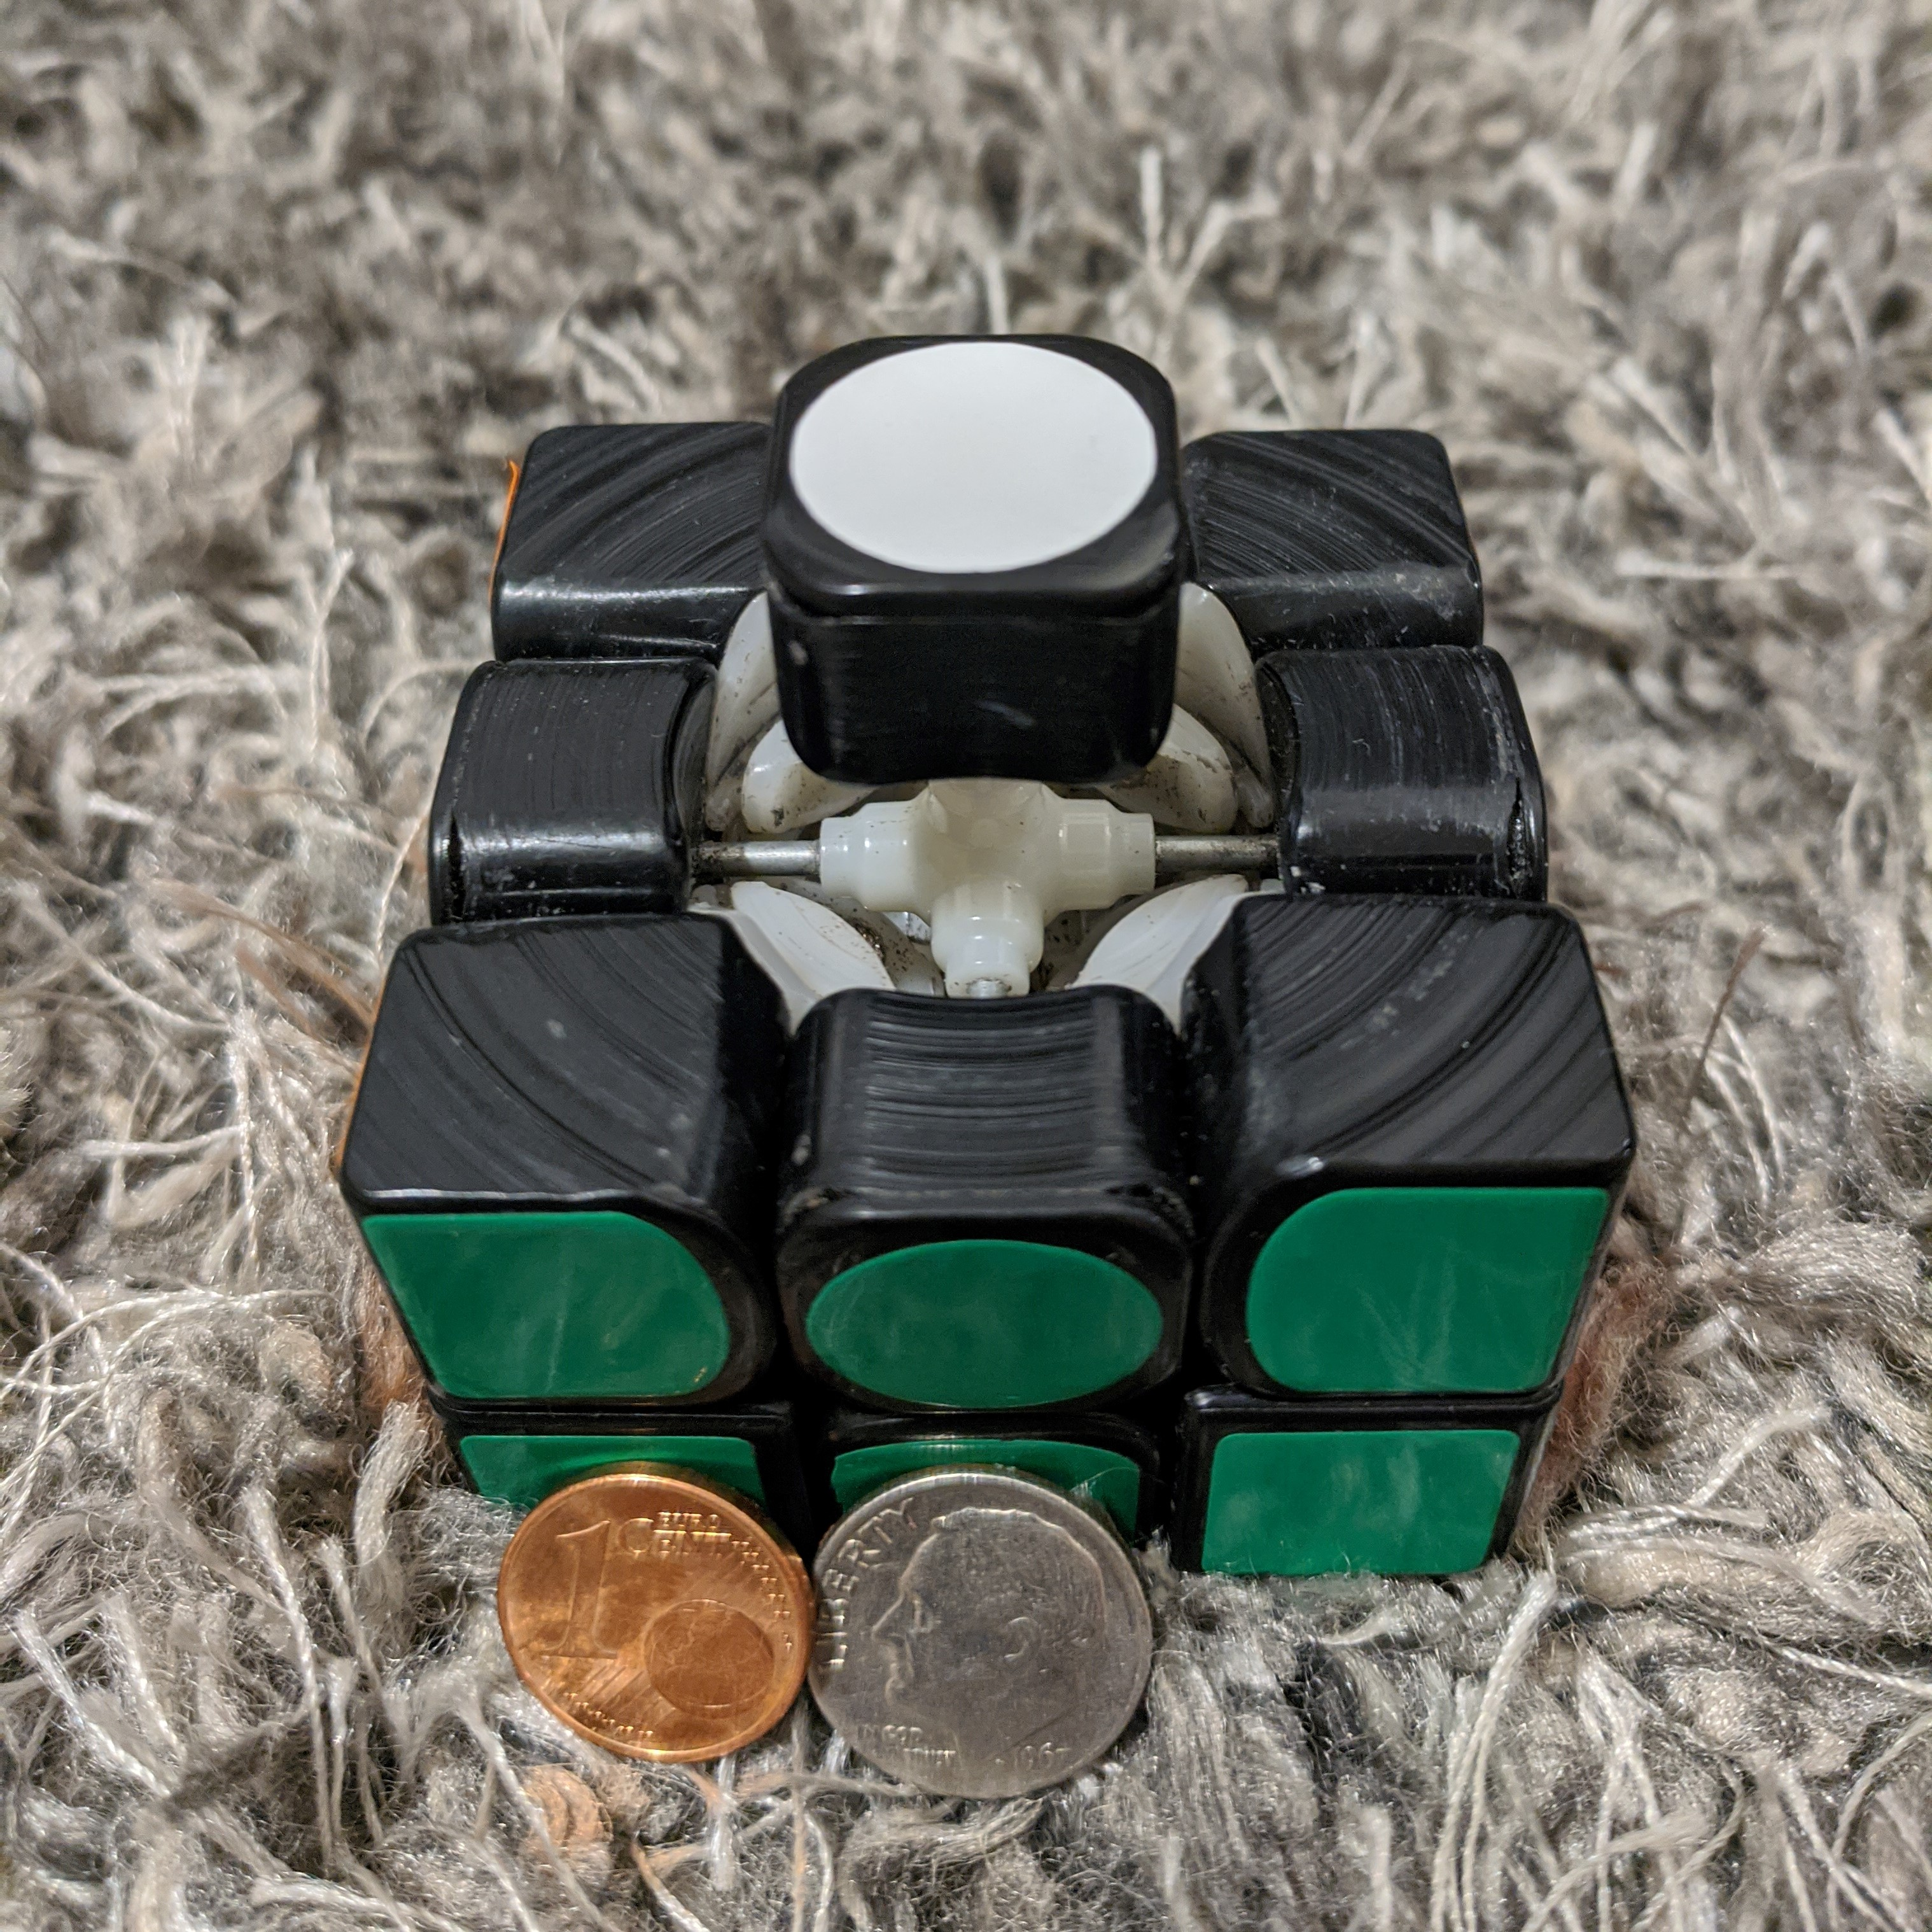
\includegraphics[width=\linewidth]{Figures/6 PCB Design/356_core_cropped.jpg}
    \end{subfigure}
    \begin{subfigure}{.45\textwidth}
        \centering
        \caption{View of the space inside the centerpiece}
        \label{fig:356-core-open}
        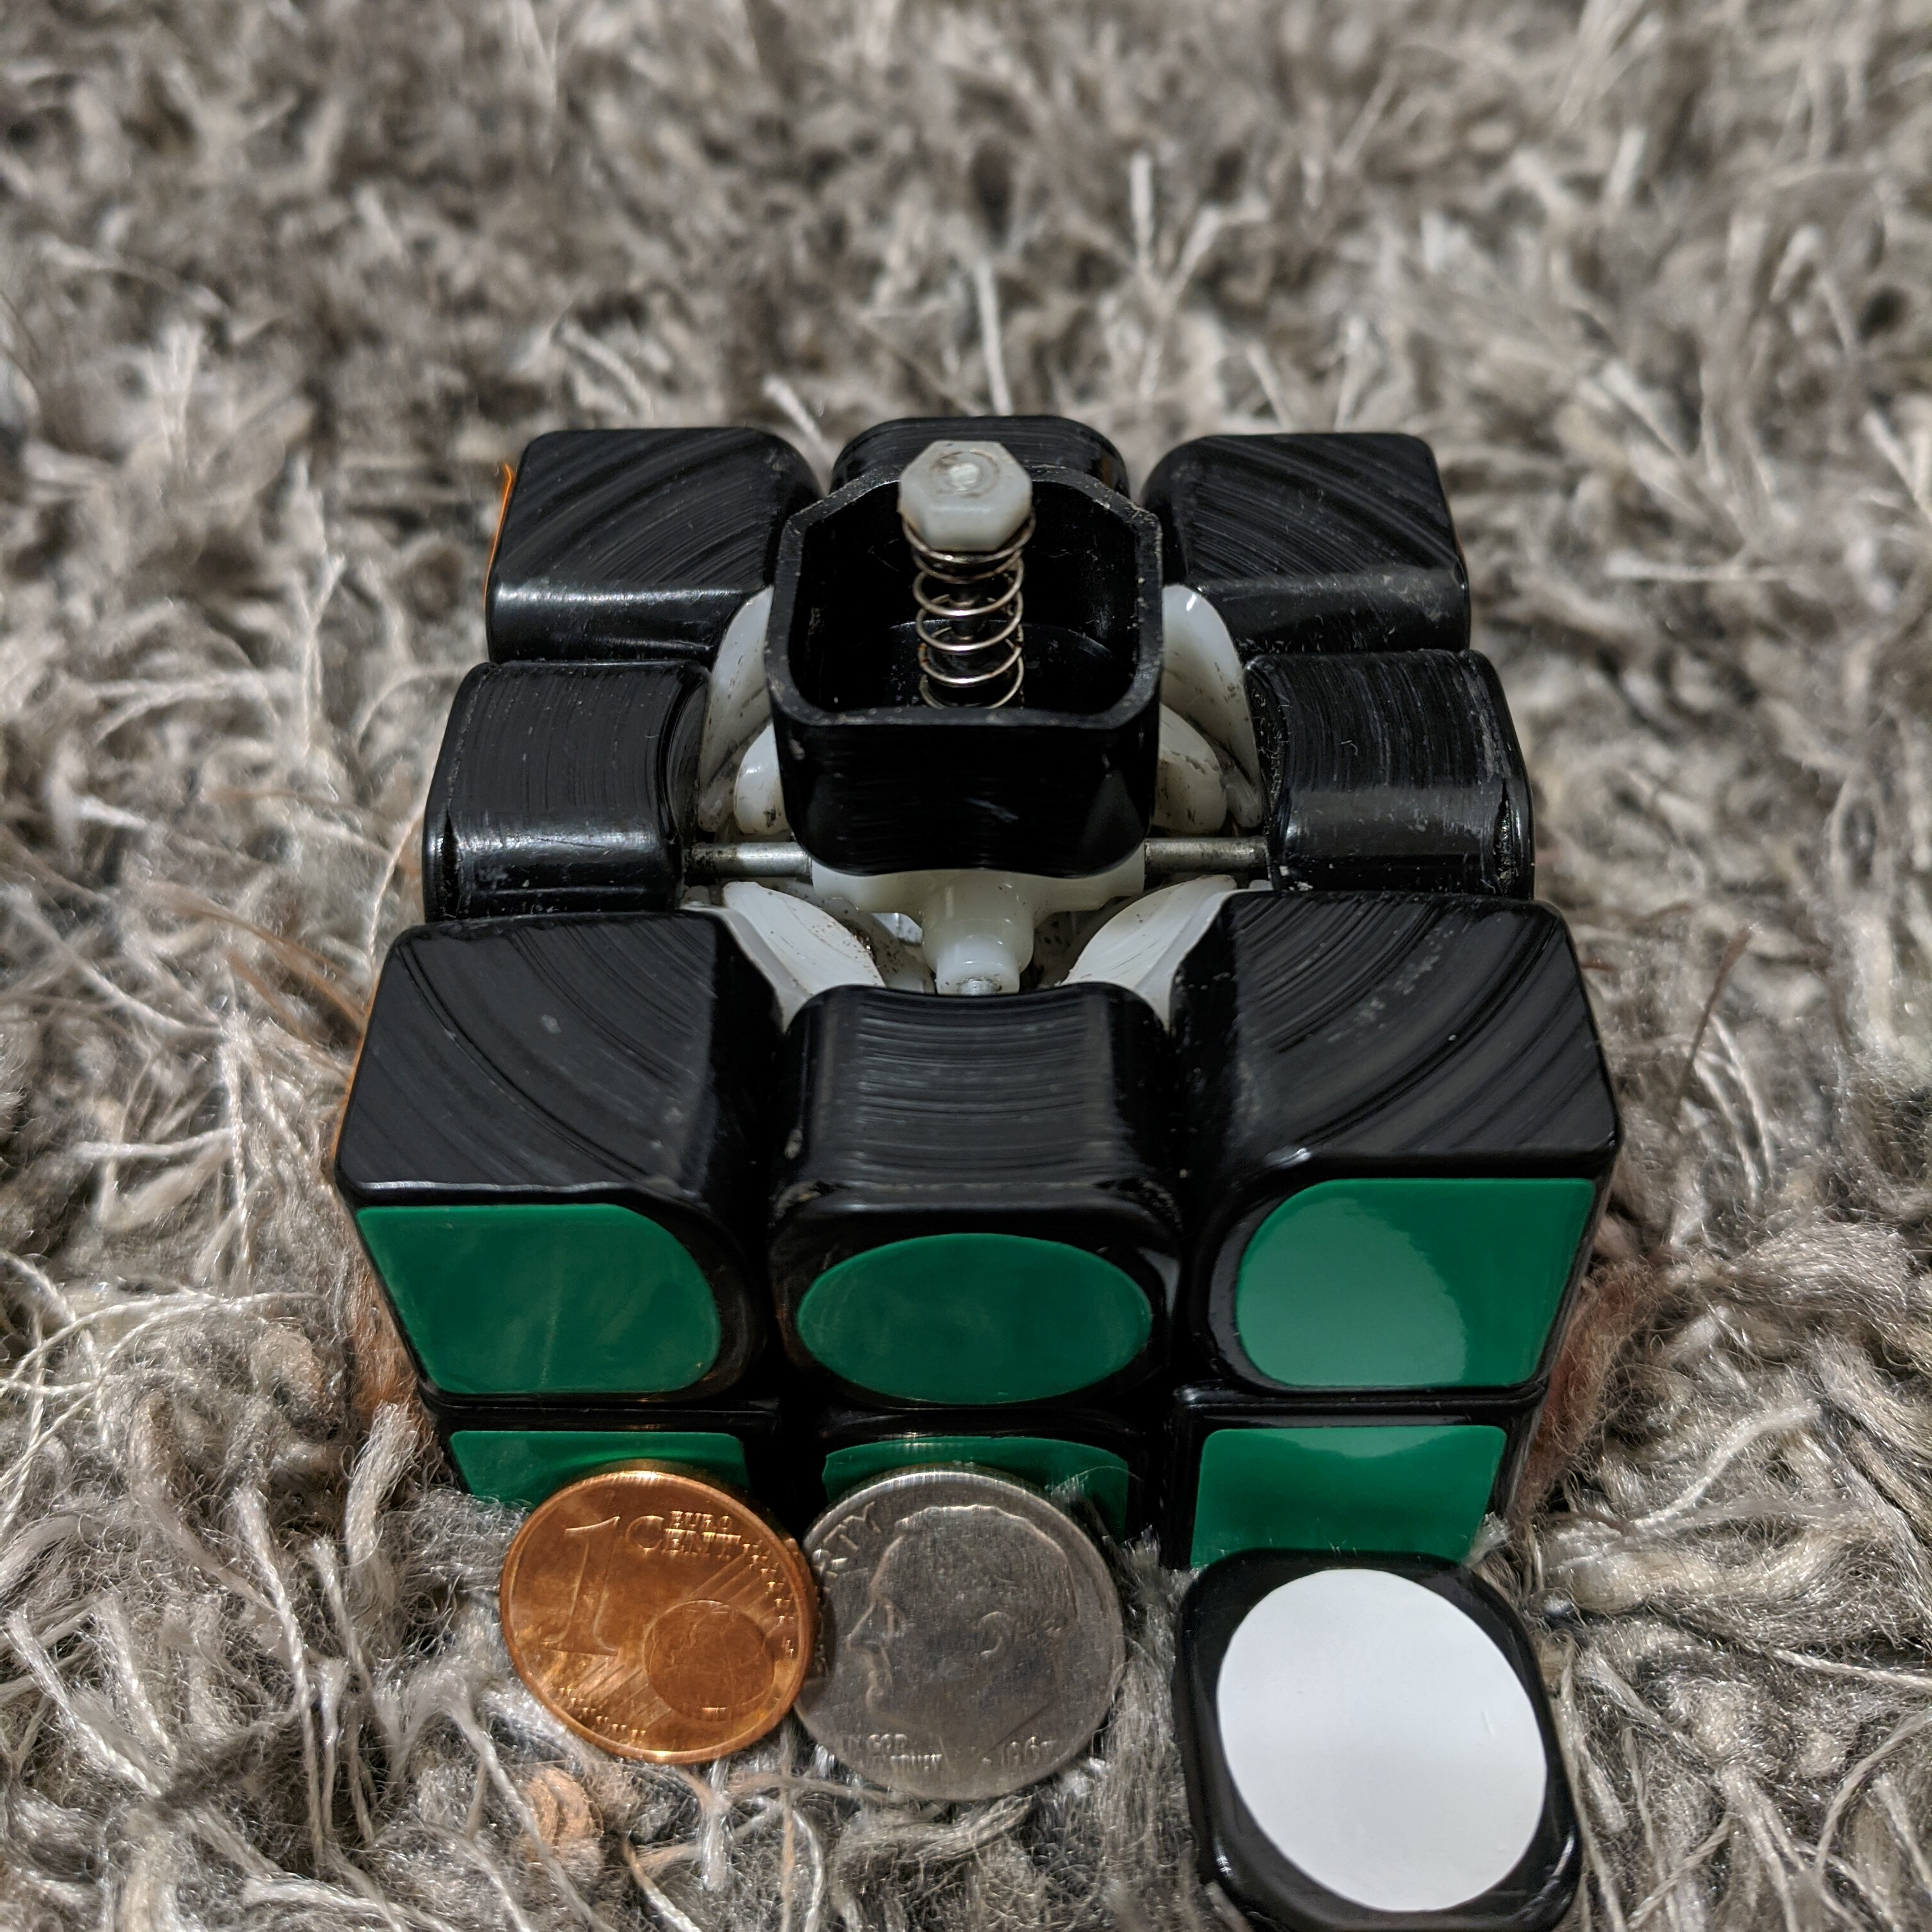
\includegraphics[width=\linewidth]{Figures/6 PCB Design/356_core_open_cropped.jpg}
    \end{subfigure}
\end{figure}

\subsection{Precision of Tone Generation}
\label{subsec:precision-of-tone-generation}

While the receiver specified in Chapter \ref{Chapter5} supports custom
state to frequency mappings, it expects that the frequency
corresponding to each centerpiece's state stays constant throughout the
entire audio recording. As such, the chosen transmitter design can
encode centerpiece states with any frequency (assuming the chosen
frequencies work within the constraints specified in Section
\ref{sec:protocol-requirements}), but it must produce its chosen
frequencies with high precision.

\subsection{Responsiveness to Face Turns}
\label{subsec:responsiveness-to-face-turns}

The chosen transmitter design must respond to an applied face turn by
changing the currently transmitted audio frequency to the frequency
corresponding to the new centerpiece state. Since top speedcubers can
reach a burst turn speed of 20 TPS (see Section
\ref{sec:alternatives}), this means this frequency change must complete
within 50ms.

\subsection{Signal-to-Noise Ratio}
\label{subsec:transmitter-signal-to-noise-ratio}

The transmitter must create tones loud enough to be easily
distinguished from ambient noise, including the sound of the Rubik's
Cube's own turns. In light of the above requirement for the transmitter
to fit within a center cubie
(\ref{subsec:prospects-of-miniaturization}), this requirement will also
require the transmitter design to consider how to overcome any audio
dampening caused by such an enclosure.


\newpage
\section{Design}
\label{sec:transmitter-design}

Given the above constrains, this section will detail a design for a
printed circuit board capable of precisely generating four distinct
tones.

\subsection{The 555 Timer}
\label{sec:the-555-timer}

The core component in this PCB design is a 555 timer, which is a
computer chip that facilitates the generation of many types of voltage
frequencies in a circuit.

For this transmitter, the 555 timer will be configured to output a
square wave voltage signal with a 50\% duty cycle (i.e. "Astable
Operation") \cite{icm7555}. This means the voltage on the output pin
will alternate between low and high, spending equal amounts of time in
each state.

The attentive reader will notice that the square wave signal proposed
here differs from the sine wave used to create the synthetic audio in
Figure \ref{fig:code-generate-alg-audio}. Valid concerns may even be
raised about the fact that a square wave is actually a composite of a
fundamental sine wave and infinitely many harmonics \cite{harmonics}.
However, since the nearest harmonic in a square wave with a 50\% duty
cycle oscillates at a frequency three times as fast as the fundamental
\cite{square-waves}, then choosing a fundamental frequency of at least
6.67kHz places the nearest harmonics beyond the range of frequencies
measurable by a typical smartphone or laptop microphone (see Section
\ref{subsec:frequency-response-range}).

The standard schematic for creating this type of voltage signal is
depicted in Figure \ref{fig:555_astable}.

\begin{figure}[h]
    \centering
    \caption{Standard 555 Timer Circuit for Astable Operation \cite{icm7555}}
    \label{fig:555_astable}
    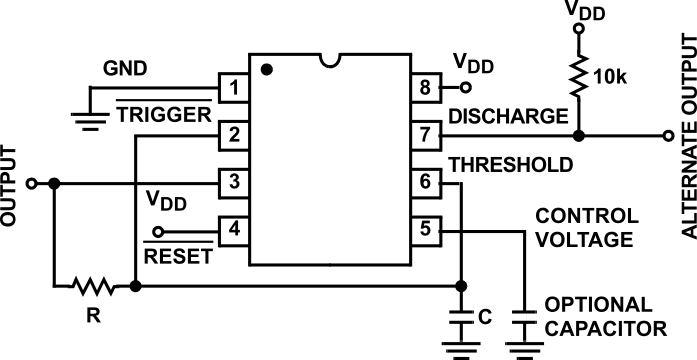
\includegraphics[width=0.75\linewidth]{Figures/6 PCB Design/555_astable.png}
\end{figure}

The two key components are the resistor \code{R} and the capacitor
\code{C} whose respective resistance and capacitance control the output
frequency \code{f} via the relation shown in Equation \ref{eq:555-freq}
\cite{icm7555}:

\begin{equation}\label{eq:555-freq}
    f = \frac{1}{1.4 R C}
\end{equation}

\subsection{Creating Audio}

The 555 timer's varying voltage output can be easily converted to
audible sound by attaching a voltage controlled speaker to the output
wire coming from pin 3 in Figure \ref{fig:555_astable}. However, this
will only produce one continuous tone, and each centerpiece will need
to be able to switch between four distinct tones. As such, the resistor
\code{R} will need to be replaced with four separate resistors (labeled
\code{R1}, \code{R2}, \code{R3}, \code{R4} in Figure
\ref{fig:555_astable_modded}) and a switch. The switch will be
connected to the cube so that a 90$^\circ$ rotation will change which
resistor is in series with the circuit, thus changing the output audio
frequency of the speaker.

\begin{figure}[h]
    \centering
    \caption{Centerpiece State Transmitter Circuit}
    \label{fig:555_astable_modded}
    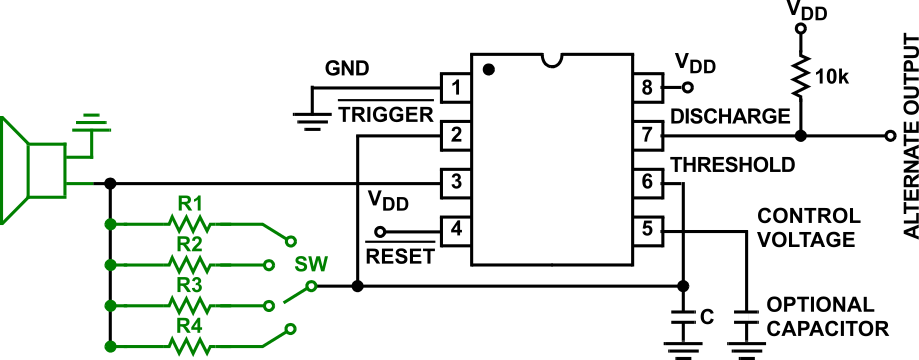
\includegraphics[width=\linewidth]{Figures/6 PCB Design/555_astable_modded.png}
\end{figure}

Alternatively, it is mathematically valid to instead switch between
four different capacitors of different capacitance. However, for the
reasons described in Section \ref{subsec:freq-selection}, opting to
switch between resistors proved more practical.

\subsection{Choosing the values of \code{R} and \code{C}}
\label{subsec:freq-selection}

\begin{sidewaysfigure}
    \centering
    \caption{Output Frequencies of Common \code{R} and \code{C} Values}
    \label{fig:freq-selection}
    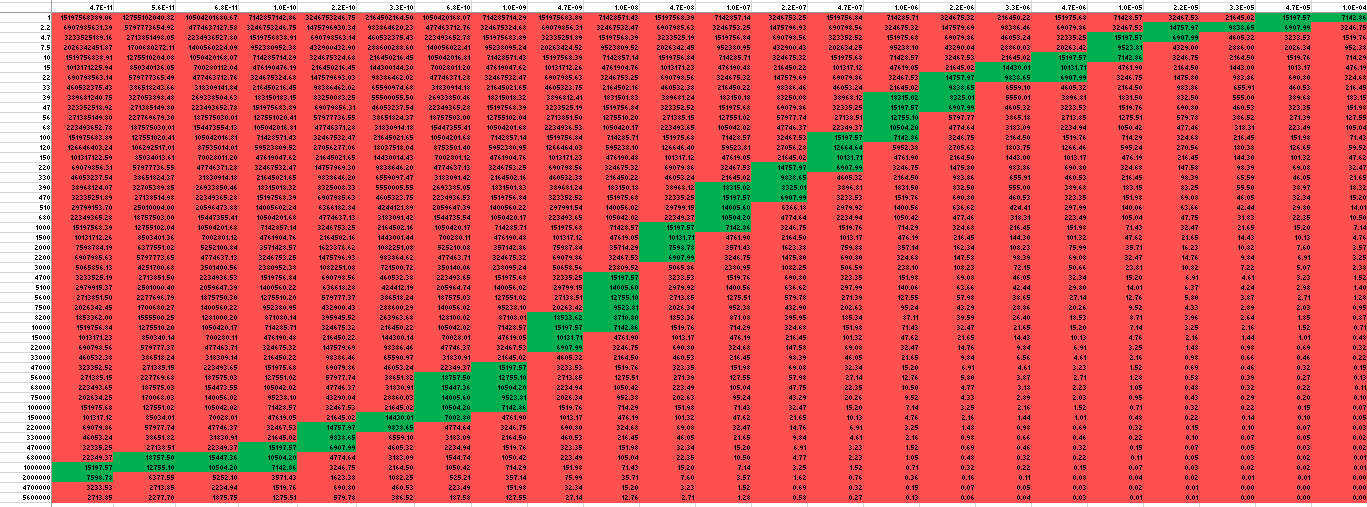
\includegraphics[width=\linewidth]{Figures/6 PCB Design/freq_selection.png}
\end{sidewaysfigure}

There are infinitely many combinations of \code{R} and \code{C} that
will produce any single desired output frequency \code{f}; however, the
set of resistances and capacitances of commonly produced resistors and
capacitors is finite. While multiple components can be combined to
produce more specific resistances and capacitances, doing so would
increase the overall component count for a circuit board that is
constrained to a small physical size. As such, this proof-of-concept
design will focus on producing frequencies attainable with a single
capacitor and resistor pair.

Since each centerpiece transmitter needs to produce four distinct
frequencies, four separate capacitor-resistor pairs are required.
However, since the output frequency can be varied by adjustments to
\emph{either} the capacitance \emph{or} resistance, one of those two
options can be held constant to reduce the overall component count.

To chose which one to hold constant, the output frequencies of all
possible pairings of capacitors and resistors from two cheap Amazon
kits \cite{amazon-capacitors} \cite{amazon-resistors} were calculated
using Equation \ref{eq:555-freq}. The resulting table was then color
coded to highlight the usable frequencies in green (6.67kHz to
20kHz)\footnote{6.67kHz is the lower bound derived in Section
\ref{sec:the-555-timer} and 20kHz the upper limit of the typical
frequency response range discussed in Section
\ref{subsec:frequency-response-range}} while leaving all other unusable
frequencies in red. The result is shown in Figure
\ref{fig:freq-selection} with the various resistances shown on the
vertical axis and the various capacitances along the horizontal axis.

A close observation of the resulting sigmoid shape of usable
frequencies reveals only one location where there are at least four
usable frequencies associated with a fixed resistance (i.e. row of
green cells), compared to ten locations where there are at least four
usable frequencies associated with a fixed capacitance (i.e. column of
green cells). As such, the most practical value to hold constant here
is the capacitance.

One of the locations with a viable fixed capacitance is shown in Figure
\ref{fig:freq-selection-r}. This pairing of a 10nF capacitor with four
resistors with respective resistances of 4.7k$\Omega$, 5.1k$\Omega$,
5.6k$\Omega$, and 7.5k$\Omega$ will be used in the prototype created in
Section \ref{sec:prototype}.

\begin{figure}[h]
    \centering
    \caption{Output Frequencies of Common \code{R} and \code{C} Values}
    \label{fig:freq-selection-r}
    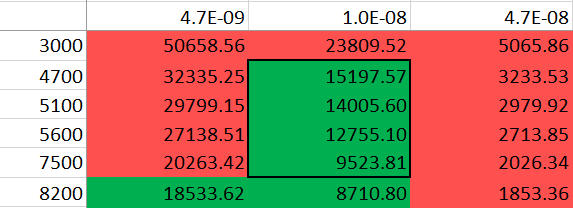
\includegraphics[width=0.8\linewidth]{Figures/6 PCB Design/freq_selection_r.png}
\end{figure}


\section{Prototyping}
\label{sec:prototype}

The key step to produce a proof-of-concept is to put everything
together on a breadboard and turn on the power while recording the
output audio to make sure four distinct tones are produced.

This step begins by gathering all the components from the schematic in
Figure \ref{fig:555_astable_modded} with the specific values of
\code{C}, \code{R1}, \code{R2}, \code{R3}, and \code{R4} shown in
Figure \ref{fig:freq-selection-r}. These components are then placed
onto a physical breadboard in accordance with the schematic's defined
layout. Connecting \code{VDD} and \code{GND} to power then causes the
speaker to produce a tone. With power still connected, the switch can
be moved to put any other resistor in series to change the resulting
tone of the speaker.

The result is shown in Figure \ref{fig:breadboard}. The left section of
the figure shows a spectrogram of the four distinct tones produced by
moving the green wire (representing the rotary switch) through each of
the four resistors on the breadboard in the right section of the figure.

\begin{figure}[h]
    \centering
    \caption{Breadboard Prototype}
    \label{fig:breadboard}
    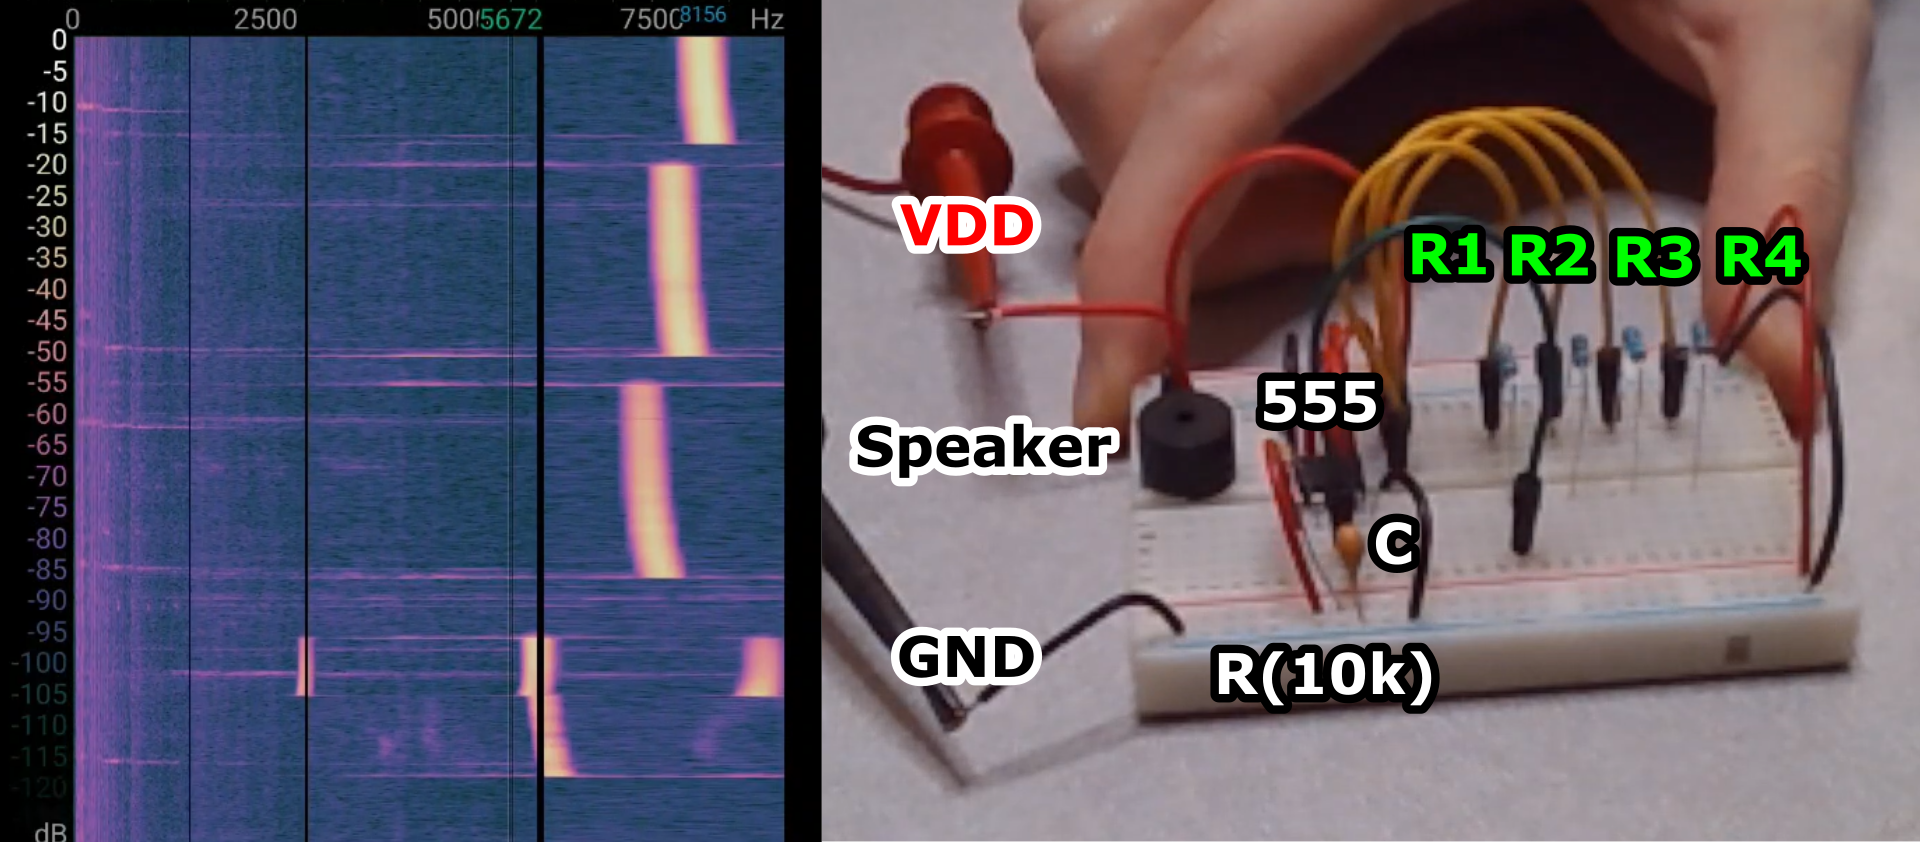
\includegraphics[width=\linewidth]{Figures/6 PCB Design/breadboard_spectrogram.png}
\end{figure}


\section{Miniaturization}

- highlight the value of so few components for the physical size
requirement, e.g. the prospects of A SMD version of the board

- If possible, create a demo in KiCAD...
- include a picture showing the dimensions of the gans 356 internal
core. Compare to the demo board in KiCad.

- Give a final part count.

- Talk about sizes for the components of the pcb.

- Discuss SMD versions

\begin{figure}[h]
    \centering
    \caption{Transmitter Circuit Inside a Custom Gans 356 Centercap}
    \label{fig:core-placement}
    \begin{subfigure}{.30\textwidth}
        \centering
        \caption{Internal View}
        \label{fig:core-circuit}
        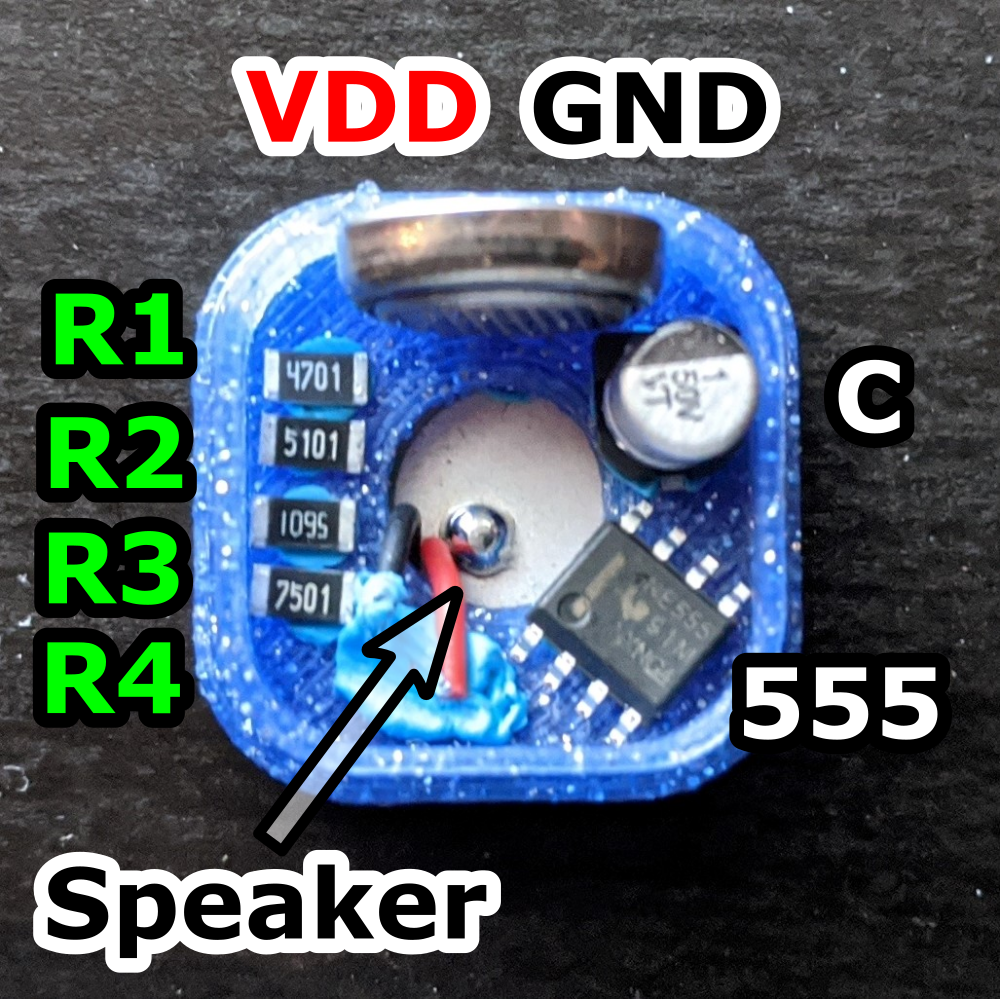
\includegraphics[width=\linewidth]{Figures/6 PCB Design/core_labelled.png}
    \end{subfigure}
    \begin{subfigure}{.30\textwidth}
        \centering
        \caption{Bird's Eye View}
        \label{fig:core-placement-birds-eye}
        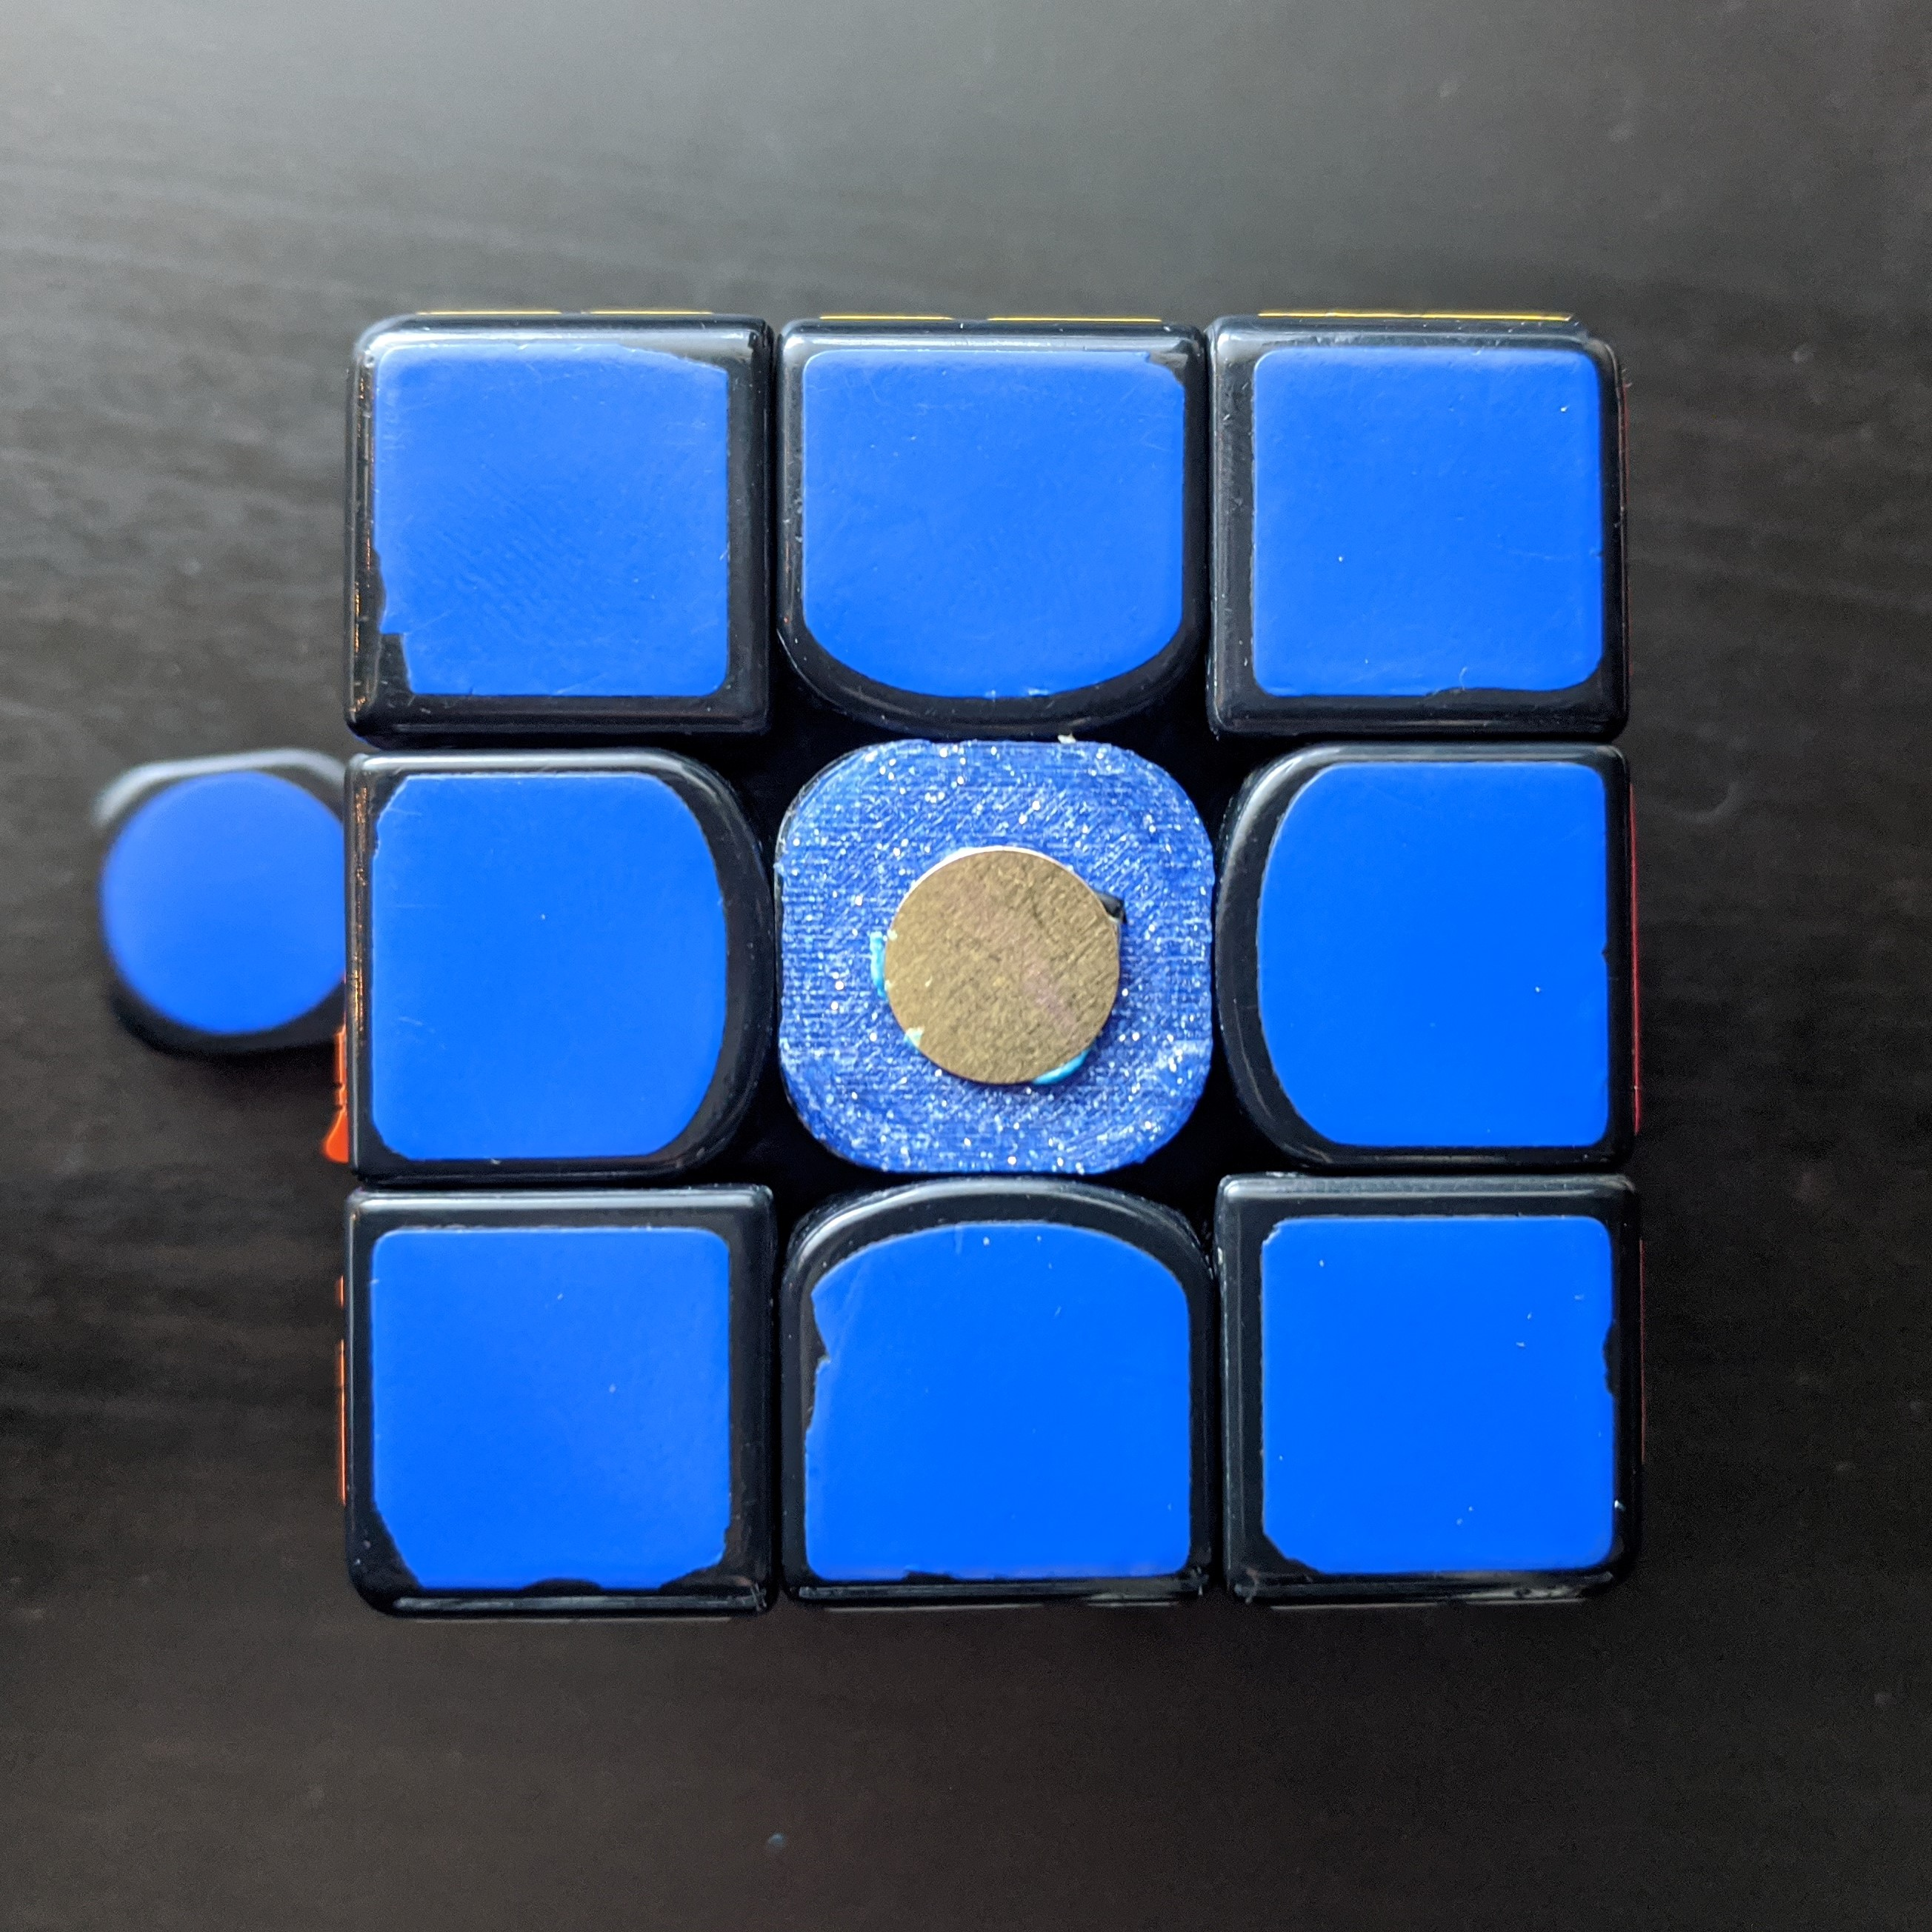
\includegraphics[width=\linewidth]{Figures/6 PCB Design/core_placement_birds_eye_square.jpg}
    \end{subfigure}
    \begin{subfigure}{.30\textwidth}
        \centering
        \caption{Isometric View}
        \label{fig:core-placement-isometric}
        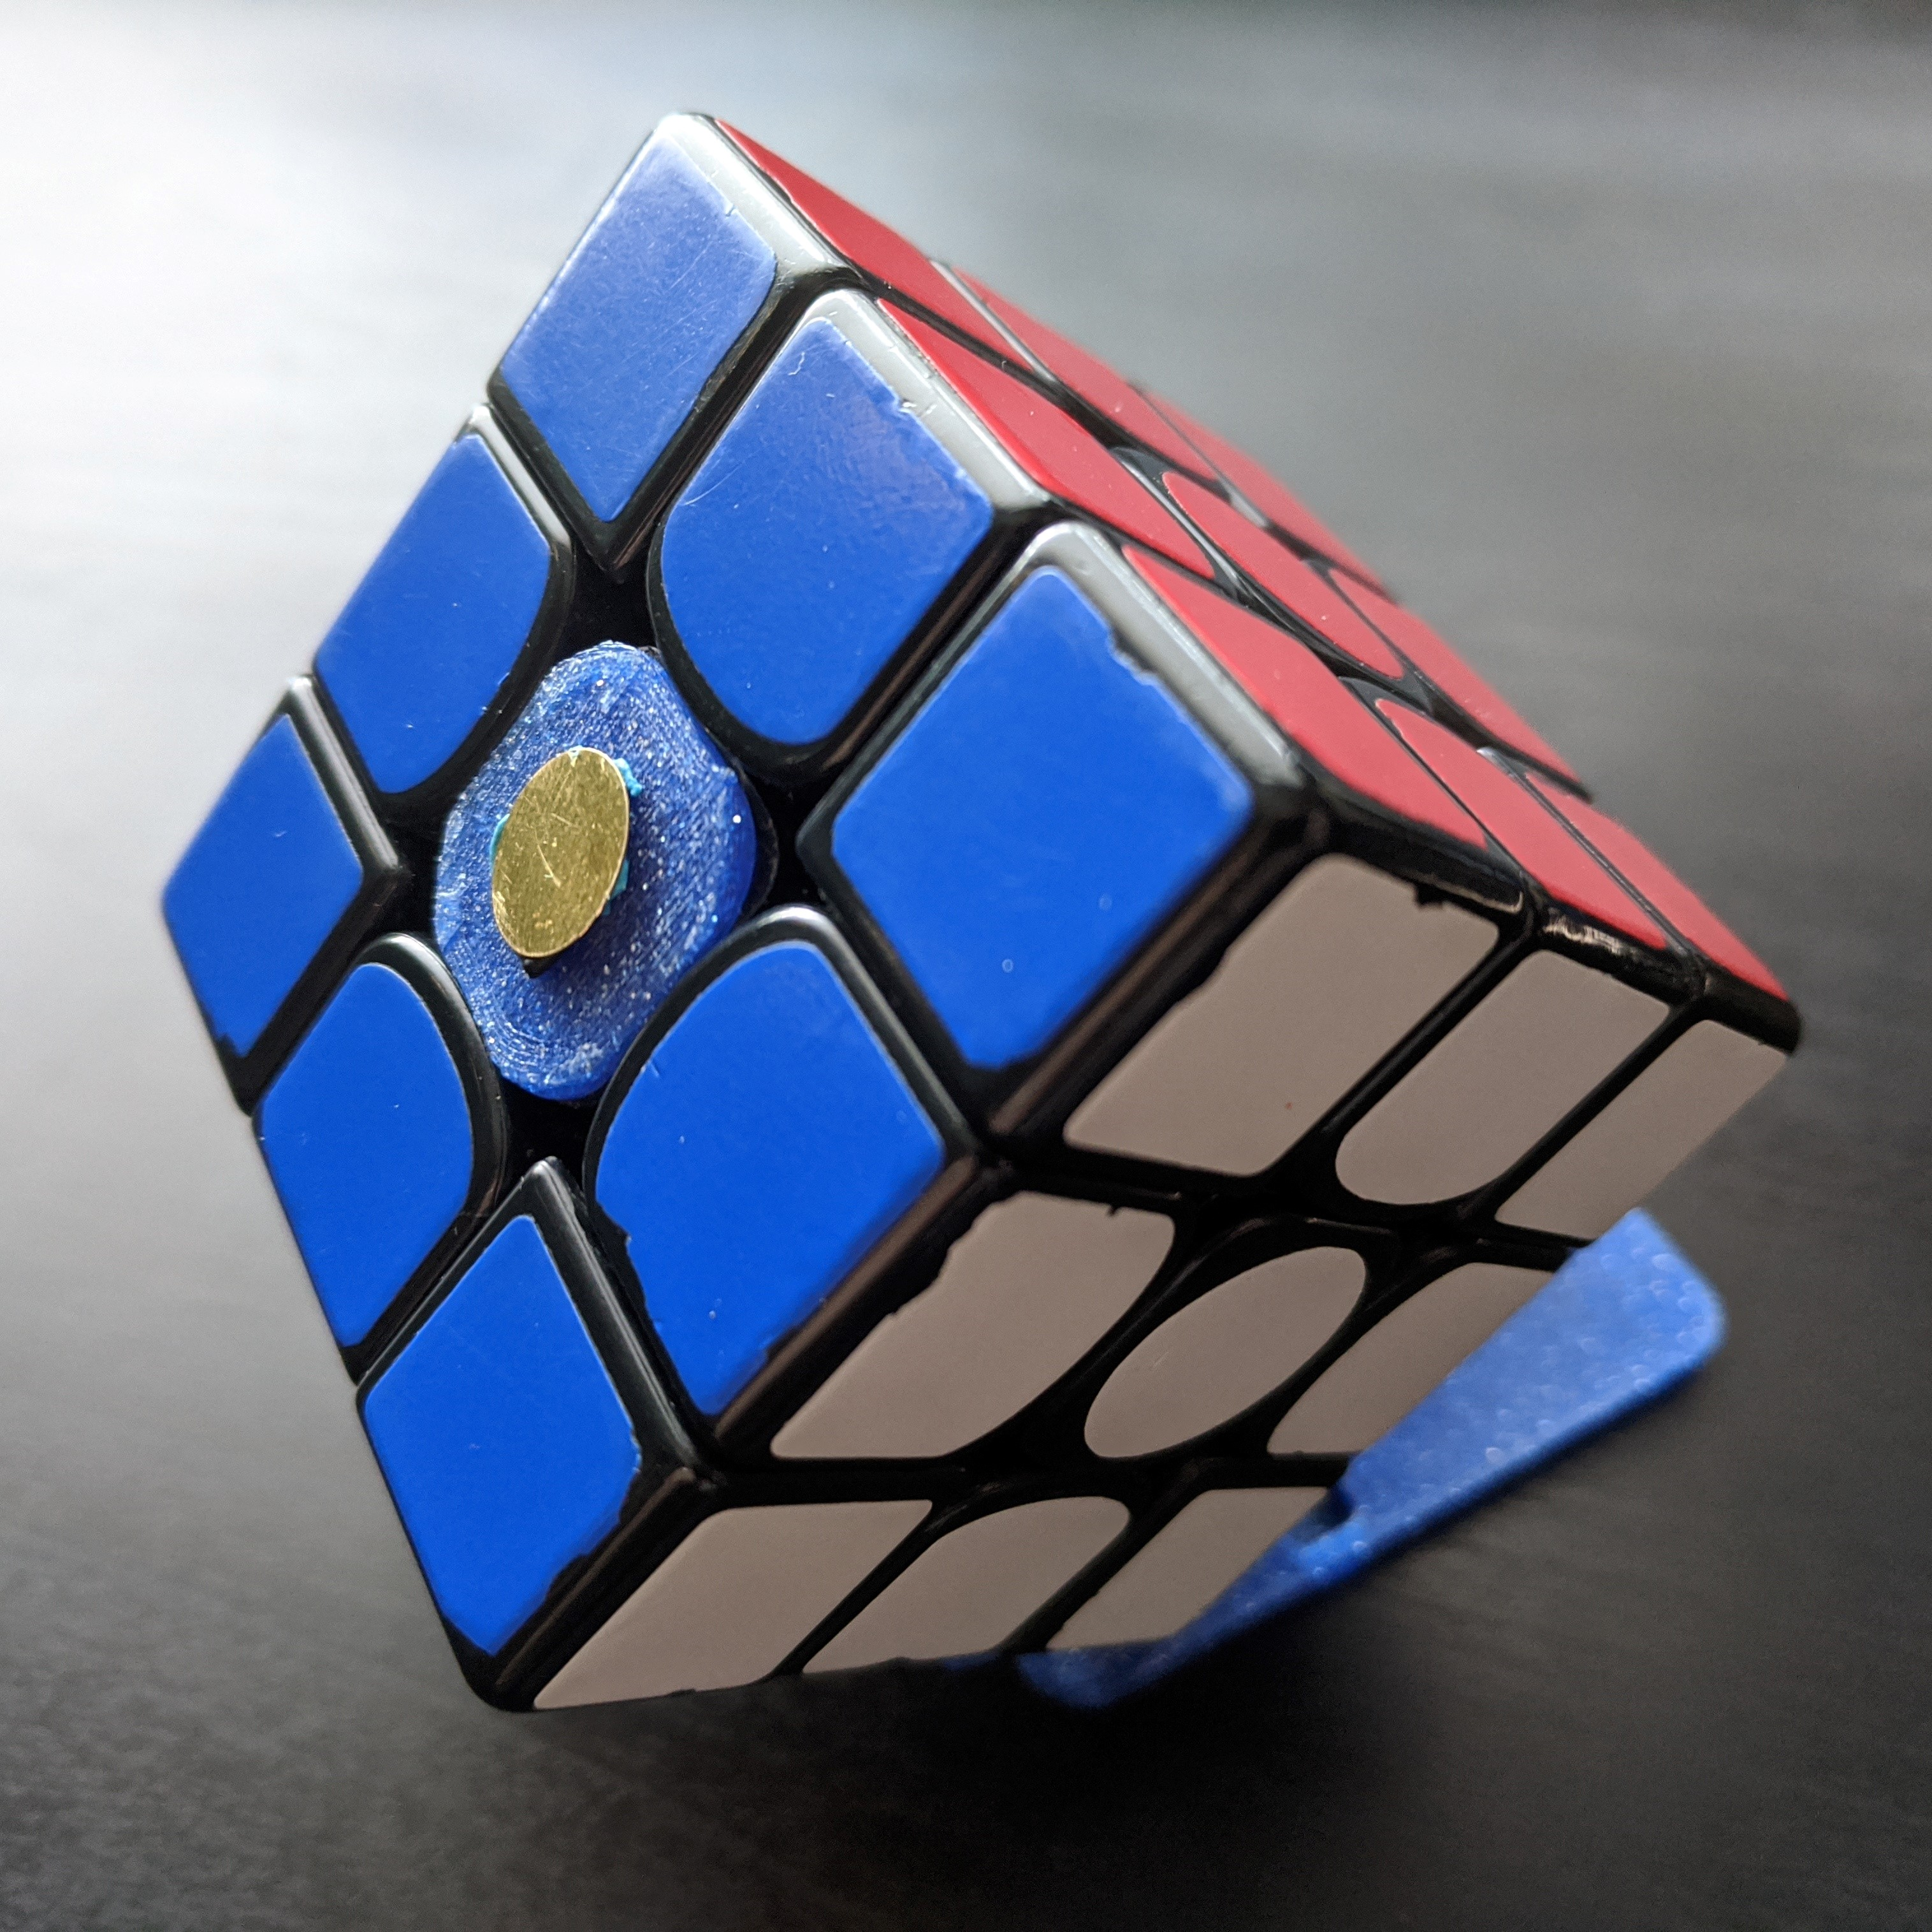
\includegraphics[width=\linewidth]{Figures/6 PCB Design/core_placement_isometric_square.jpg}
    \end{subfigure}
\end{figure}

\section{Minimizing Sound Obstruction}
Section \ref{subsubsec:key-observations-from-the-spectrogram} talks about the noise levels from various speedcubes. Constrast with the noise levels produced here to show validity.

TODO Discuss the "tupperware" tests -> design of various center caps.

\section{Summary}
